\chapter {Các công trình nghiên cứu liên quan}
\label{chp:03}

Chương này trình bày các công trình tiêu biểu trong ba hướng nghiên cứu liên quan đến đề tài: (i) các vi xử lý mã nguồn mở dựa trên RISC-V cho ứng dụng Edge AI, (ii) các framework gia tốc CNN trên FPGA, và (iii) các kiến trúc mạng nơ-ron và kỹ thuật lượng tử hóa hiệu quả cho thiết bị biên. Phần kết của mỗi mục sẽ làm rõ vị trí thiết kế của đề tài so với từng hướng tiếp cận đã có.

%=================================================================================
\section{Vi xử lý mã nguồn mở RISC-V cho Edge AI}
\label{sec:riscv_related}

\subsection{Hệ sinh thái PULP và Pulpissimo}
PULPissimo (PULP Independent Single-stream Shared-memory Integrated Subsystem) là một SoC vi điều khiển 32-bit dựa trên RISC-V, được phát triển bởi nhóm PULP (Parallel Ultra Low Power) thuộc ETH Zürich và Đại học Bologna \cite{pulpissimo}. Pulpissimo cung cấp một nền tảng phần cứng tiết kiệm năng lượng nhưng vẫn đảm bảo hiệu năng tính toán cho IoT và Edge AI, bao gồm: lõi RI5CY (tên cũ của CV32E40P), hệ thống bộ nhớ TCDM 16-bank, bộ điều khiển uDMA cho ngoại vi, hệ thống ngắt, và giao diện Hardware Processing Engine (HWPE) cho các bộ tăng tốc tùy chỉnh.

Đề tài này \textbf{kế thừa lõi xử lý CV32E40P từ Pulpissimo} (qua submodule chính thức của OpenHW Group) nhưng \textbf{không sử dụng các thành phần khác} của Pulpissimo: thay vì TCDM 16-bank + Logarithmic Interconnect, đề tài thiết kế lại memory subsystem theo chuẩn AXI4 của Xilinx (dual-port BRAM + AXI SmartConnect). Lựa chọn này nhằm tích hợp tự nhiên với Vivado IP Catalog và đồng bộ địa chỉ logic giữa ARM và RISC-V (xem mục~\ref{sec:pl_design}).

\subsection{Mở rộng tập lệnh RISC-V cho mạng nơ-ron}
Một hướng tiếp cận để gia tốc mạng nơ-ron trên RISC-V là can thiệp trực tiếp vào kiến trúc tập lệnh (ISA Extensions). Công trình \textit{``FPGA-Accelerated RISC-V ISA Extensions for Efficient Neural Network Inference on Edge Devices''} \cite{parameshwara2025fpga} là một minh chứng tiêu biểu cho trường phái thiết kế \textit{tightly-coupled}: thay vì tách bộ tăng tốc thành IP độc lập, nhóm tác giả định nghĩa các chỉ thị MAC INT8 mới, tích hợp ngay vào pipeline ALU của lõi RISC-V.

\textbf{Ưu điểm} của hướng này là độ trễ giao tiếp gần như bằng 0 (không qua bus AXI) và tiết kiệm năng lượng do không phải đọc/ghi bộ nhớ ngoài. \textbf{Nhược điểm}: (i) đòi hỏi can thiệp sâu vào RTL của CPU, có rủi ro làm giảm Fmax; (ii) bị giới hạn bởi băng thông tập thanh ghi 32-bit, khó scale lên các layer lớn; (iii) cần custom GCC/LLVM toolchain để biên dịch các lệnh tùy biến.

\textbf{Đối chiếu với đề tài:} Đề tài chọn hướng \textit{loosely-coupled} (Conv-CNN là IP độc lập giao tiếp qua AXI), đánh đổi độ trễ giao tiếp lấy tính module hóa và khả năng scale. Lõi RISC-V CV32E40P được giữ nguyên bản (RV32IMC standard), không cần custom toolchain -- ưu tiên tính bảo trì và tái sử dụng cho các capstone project sau.

%=================================================================================
\newpage
\section{Framework gia tốc CNN trên FPGA}
\label{sec:fpga_frameworks}

Phần này tổng hợp 4 framework tiêu biểu cho việc gia tốc CNN trên FPGA, được lựa chọn dựa trên mức độ phù hợp với platform của đề tài (Xilinx Zynq UltraScale+) và tính đại diện cho các trường phái thiết kế khác nhau.

\subsection{Vitis AI DPU (Xilinx)}
Vitis AI Deep Processing Unit (DPU) là giải pháp thương mại của Xilinx (nay là AMD-Xilinx) dành cho việc triển khai CNN trên dòng SoC Zynq UltraScale+ (bao gồm Kria KV260) \cite{vitis_ai}. DPU được phân phối dưới dạng IP đóng (encrypted bitstream), kèm theo compiler chuyển mô hình từ TensorFlow/PyTorch sang chỉ thị máy của DPU. Người dùng chỉ cần quantize mô hình và gọi runtime API, không cần thiết kế RTL.

\textbf{Đối chiếu với đề tài:} DPU cho phép triển khai nhanh nhiều mô hình lớn (ResNet, MobileNet, YOLO) nhưng có ba hạn chế đáng kể: (i) \textit{closed-source} -- không thể tùy biến op set hay quantization scheme; (ii) tài nguyên cố định -- DPU B1024/B2048 chiếm phần lớn FPGA, khó nhường chỗ cho RISC-V soft-core; (iii) không có khả năng \textit{hardware-software co-design} ở mức RTL -- yếu tố cốt lõi của đề tài. Đề tài chấp nhận phạm vi op nhỏ hơn nhưng đổi lấy tính kiểm soát hoàn toàn pipeline phần cứng.

\subsection{FINN -- HLS-based BNN Accelerator (Xilinx Research)}
FINN \cite{finn_paper} là framework do Xilinx Research phát triển, sinh tự động bộ tăng tốc cho Binarized Neural Networks (BNN, weights/activations 1-bit) qua Vivado HLS. FINN tận dụng đặc điểm BNN -- thay phép tích chập bằng XNOR + Popcount thực hiện hoàn toàn bằng LUT -- để đạt throughput cao mà không tốn DSP.

\textbf{Đối chiếu với đề tài:} BNN cho phép throughput cực cao (hàng nghìn img/s) nhưng giảm độ chính xác đáng kể trên các tập dữ liệu phức tạp. Đề tài chọn INT8 (đề xuất bởi Jacob et al. \cite{jacob2018quantization}) làm điểm cân bằng tốt hơn giữa chính xác và hiệu năng cho bài toán phân loại nhị phân, đồng thời tận dụng được DSP48E2 của Ultrascale+ (vốn dồi dào: 1248 DSP trên KV260).

\subsection{hls4ml (CERN -- Fermilab Collaboration)}
hls4ml \cite{hls4ml} là framework do nhóm vật lý hạt nhân (CERN, Fermilab) phát triển ban đầu cho ứng dụng trigger LHC, nay được mở rộng cho Edge AI. hls4ml nhận mô hình Keras/PyTorch làm đầu vào và sinh ra C++ HLS code, sau đó qua Vivado HLS để tổng hợp thành RTL. Toàn bộ mạng được \textit{fully unrolled} thành dataflow pipeline, đạt độ trễ rất thấp (microsecond range).

\textbf{Đối chiếu với đề tài:} hls4ml hoàn toàn HLS-based, không có CPU tham gia điều phối -- mô hình bị ``cứng hóa'' thành RTL, đổi mô hình phải re-synthesize bitstream. Đề tài giữ kiến trúc phân tầng với RISC-V làm orchestrator: đổi mô hình chỉ cần thay \texttt{layer\_table.h} + \texttt{weights.bin}, không cần re-synth -- phù hợp hơn với mục tiêu prototyping nhanh nhiều mô hình.

\subsection{CFU Playground (Google)}
CFU Playground \cite{cfu_playground} là project mã nguồn mở của Google, kết hợp lõi RISC-V (VexRiscv) với Custom Function Unit (CFU) trên FPGA, chạy TensorFlow Lite Micro. CFU là một dạng \textit{tightly-coupled} accelerator: được thêm vào ALU của RISC-V qua chỉ thị tùy biến, gần giống hướng tiếp cận của \cite{parameshwara2025fpga}.

\textbf{Đối chiếu với đề tài:} CFU Playground và đề tài đại diện cho hai trường phái song song trong nghiên cứu RISC-V + AI:
\begin{itemize}
    \item \textbf{CFU Playground (tightly-coupled):} Bộ tăng tốc nằm trong lõi CPU, chia sẻ register file. Phù hợp khi mô hình nhỏ và op đơn giản (thường ở mức MAC vector).
    \item \textbf{Đề tài (loosely-coupled):} Bộ tăng tốc là IP độc lập giao tiếp qua AXI và DMA. Phù hợp khi op phức tạp (Conv 3$\times$3 với line buffer + window + requantize) và cần streaming bandwidth cao từ DDR.
\end{itemize}
Lựa chọn của đề tài nghiêng theo hướng loosely-coupled vì: (i) op chính là Conv 3$\times$3 với line buffer 16~KB BRAM -- không thể nhét vào trong CPU; (ii) cần DMA tốc độ cao từ DDR mà CFU không hỗ trợ trực tiếp.

\subsection{Bảng tổng hợp so sánh}
\begin{table}[!h]
    \centering
    \caption{So sánh đa chiều các framework gia tốc CNN trên FPGA.}
    \label{tab:framework_comparison}
    \resizebox{\textwidth}{!}{%
    \begin{tabular}{|l|c|c|c|c|c|}
    \hline
    \textbf{Framework} & \textbf{Mã nguồn} & \textbf{Coupling} & \textbf{Quantization} & \textbf{Đổi mô hình} & \textbf{Có RISC-V?} \\ \hline
    Vitis AI DPU       & Closed   & Loosely (DPU IP)        & INT8           & Compile lại model    & Không (chỉ ARM) \\ \hline
    FINN               & Open     & Loosely (HLS-gen IP)    & 1-bit (BNN)    & Re-synthesize        & Không           \\ \hline
    hls4ml             & Open     & N/A (fully unrolled)    & FP/INT tùy chọn & Re-synthesize       & Không           \\ \hline
    CFU Playground     & Open     & Tightly (in-CPU)        & INT8 (TFLM)    & Re-compile firmware  & Có (VexRiscv)   \\ \hline
    \textbf{Đề tài}    & Open     & Loosely (AXI IP)        & INT8 (TFLite)  & Thay weights+table   & Có (CV32E40P)   \\ \hline
    \end{tabular}%
    }
\end{table}

%=================================================================================
\newpage
\section{Mô hình hiệu quả cho thiết bị biên}
\label{sec:efficient_models}

Bên cạnh các vi xử lý mở và framework FPGA, hướng nghiên cứu thứ ba để đưa AI lên thiết bị biên là tối ưu hóa kiến trúc mạng nơ-ron thay vì phần cứng. Hai trường phái tiêu biểu được tóm tắt dưới đây để làm rõ vị trí thiết kế của đề tài.

\paragraph{Mạng nơ-ron Nhị phân (BNN).} Courbariaux và cộng sự \cite{bnn_courbariaux} đã chứng minh khả năng huấn luyện các mạng nơ-ron sâu với trọng số và kích hoạt ép buộc về $\{+1, -1\}$ (1-bit). Lợi thế lớn nhất của BNN trên FPGA là phép tích chập được thay bằng phép logic XNOR + Popcount, có thể thực hiện trực tiếp bằng LUT mà không cần DSP. Tuy nhiên, BNN gặp giảm độ chính xác đáng kể trên các tập dữ liệu phức tạp (ImageNet). Đồ án tham khảo nguyên lý tối ưu phần cứng của BNN nhưng lựa chọn lượng tử hóa INT8 chuẩn TFLite \cite{jacob2018quantization} để đạt cân bằng tốt hơn giữa độ chính xác và hiệu năng.

\paragraph{MobileNet và Depthwise Separable Convolution.} Howard và cộng sự \cite{mobilenet_v1} đề xuất kiến trúc MobileNet sử dụng \textit{depthwise separable convolution} (tách Conv $K \times K$ thành Depthwise Conv + Pointwise $1 \times 1$) để giảm khoảng 8--9 lần số phép MAC so với Conv chuẩn cùng kích thước. MobileNet trở thành kiến trúc chuẩn cho thị giác máy trên thiết bị di động. Tuy nhiên, depthwise convolution có \textit{dataflow ngược} so với Conv chuẩn (mỗi cin $\to$ 1 output thay vì sum across cin), đòi hỏi MUX adder tree riêng và chế độ FSM mới ở bộ tăng tốc. Trong phạm vi đồ án, đề tài chọn kiến trúc \texttt{vgg-tiny} đơn giản hơn (chỉ Conv $3 \times 3$ chuẩn) để tập trung vào việc kiểm chứng đồng thiết kế phần cứng-phần mềm; hỗ trợ depthwise được dành cho hướng phát triển tiếp theo.

%=================================================================================
\section{Lượng tử hóa và huấn luyện mạng nơ-ron}
\label{sec:quantization_theory}

Trong các hệ thống học sâu truyền thống, việc huấn luyện và suy luận thường được
thực hiện trên định dạng số thực dấu phẩy động 32-bit (Float32) để đảm bảo độ chính xác cao nhất. Tuy nhiên, trên các thiết bị biên (Edge Devices) với tài nguyên hạn chế như FPGA hay vi xử lý nhúng RISC-V, các phép toán số thực tiêu tốn quá nhiều tài nguyên phần cứng và năng lượng.

Để giải quyết vấn đề này, đồ án áp dụng phương pháp lượng tử hóa số nguyên
được đề xuất bởi \textit{Jacob et al.} (Google) trong công trình
\textit{"Quantization and Training of Neural Networks for Efficient
Integer-Arithmetic-Only Inference"} \cite{jacob2018quantization}.

\begin{figure}[!h]
    \centering
    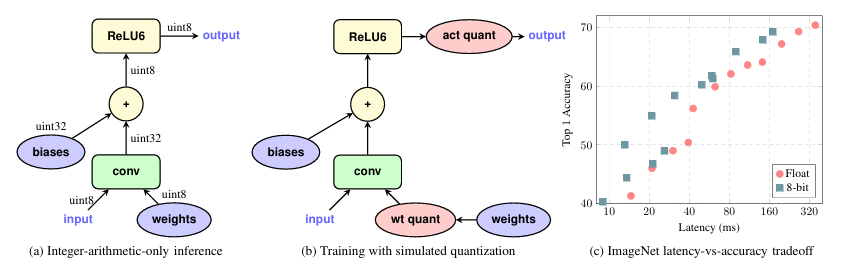
\includegraphics[width=1\linewidth]{chapter03/img/quanti.png}
    \caption{Quy trình lượng tử hóa và huấn luyện mạng nơ-ron theo Jacob et al.}
    \label{fig:quantization_process}
\end{figure}

\subsection{Cơ chế Lượng tử hóa Affine (Affine Quantization Scheme)}
Khác với các phương pháp lượng tử hóa logarit hay nhị phân, phương pháp của Jacob et al. sử dụng ánh xạ tuyến tính (Affine mapping) để chuyển đổi giữa giá trị thực ($r$) và giá trị nguyên 8-bit ($q$). Công thức ánh xạ được định nghĩa như sau:

\begin{equation}
    r = S \times (q - Z)
\end{equation}

Trong đó:
\begin{itemize}
    \item $r$ (Real value): Giá trị thực cần biểu diễn.
    \item $q$ (Quantized value): Giá trị nguyên 8-bit ($q \in [0, 255]$ hoặc $[-128, 127]$).
    \item $S$ (Scale factor): Hằng số tỉ lệ (dạng Float32 dương), xác định bước nhảy của lượng tử hóa.
    \item $Z$ (Zero-point): Giá trị nguyên đóng vai trò là điểm "0" của số thực. Điều này cho phép biểu diễn chính xác giá trị 0 thực tế (thường xuất hiện trong Padding hoặc ReLU) bằng một số nguyên, giúp duy trì độ chính xác của mạng.
\end{itemize}

Từ công thức trên, quá trình nhân chập (Convolution) giữa đầu vào $x$ và trọng số $w$ có thể được viết lại hoàn toàn dưới dạng số nguyên:

\begin{equation}
    y = \sum (x \times w) \approx S_y \left( \sum (q_x - Z_x)(q_w - Z_w) + Z_y \right)
\end{equation}

\subsection{Suy luận chỉ dùng số học nguyên (Integer-Arithmetic-Only Inference)}
Điểm đột phá trong nghiên cứu của Jacob et al. là kỹ thuật xử lý tham số $S$ (Scale). Mặc dù $S$ là số thực, nhưng trong quá trình suy luận, tích của các Scale ($M = S_x S_w / S_y$) được xấp xỉ bằng một phép nhân số nguyên và phép dịch bit (Bit-shift):

\begin{equation}
    M \approx 2^{-n} \times M_0 \quad (\text{với } M_0 \text{ là số nguyên cố định})
\end{equation}

Kỹ thuật này cho phép loại bỏ hoàn toàn khối xử lý số thực (FPU) khỏi phần cứng.
Mọi phép tính từ tích chập, cộng bias đến hàm kích hoạt đều được thực hiện bằng
các đơn vị số học nguyên (ALU Integer) và các bộ dịch bit. Đề tài hiện thực trực tiếp công thức này trong module \texttt{requantize.sv} với pipeline 3-tầng (mục~\ref{ssec:requantize}).
